% ---------------------------------------------------------------------------
% REVISION DRAFT (v2) of the manuscript rejected at TASLP prescreening,
% 10 Oct 2026. The submitted version is ../taslp/taslp.tex and is unchanged.
% All sections are consistent with the EXISTING (per-layer) data. The
% end-to-end sweep is pending; see the PENDING note in Sec. III-B.
%
% Original header: IEEE/ACM TASLP submission. No deadline; no page limit up to 10 pages, beyond
% which IEEE mandatory overlength charges apply ($200+/page). Voluntary page
% charges are explicitly NOT a prerequisite for publication, so staying within
% 10 pages makes this free to publish on the traditional (non-OA) route.
%
% Grown from paper/icassp/icassp2027.tex, which is the 5-page conference-length
% compression of the same work. Material cut there purely for space belongs
% back here.
% ---------------------------------------------------------------------------
\documentclass[journal]{IEEEtran}
\usepackage{amsmath,amssymb,graphicx,booktabs,url,tipa}
\usepackage[T1]{fontenc}
% hyperref last, so it can patch the other packages' cross-referencing.
% hidelinks: no coloured frames, which IEEE styles do not want in print;
% breaklinks: a URL split across two lines stays one clickable target, which
% both URLs in this paper are.
\usepackage[hidelinks,breaklinks=true]{hyperref}

\newcommand{\talg}{\ensuremath{t_{\mathrm{alg}}}}
\newcommand{\tcmp}{\ensuremath{t_{\mathrm{cmp}}}}
\newcommand{\tbuf}{\ensuremath{t_{\mathrm{buf}}}}

\title{Future-Context Requirements for Streaming Accent Conversion:\\
A Controlled Study Using Causal Phone Translation}
\author{Dipesh~Tripathi%
\thanks{D. Tripathi is with the University of South Dakota, Vermillion, SD,
USA (e-mail: dipesh.tripathi@coyotes.usd.edu).}%
\thanks{Harness, causality audit, sweep configurations, analysis scripts with
self-tests and per-condition hypothesis dumps:
\url{https://github.com/Dipeshtripathi13/streaming-fac-lookahead}. Data is
L2-ARCTIC~\protect\cite{l2arctic2018} via \texttt{KoelLabs/L2Arctic}. Given
that corpus's CC-BY-NC-4.0 licence, we conservatively release configurations
rather than model weights.}}

\begin{document}
% Suppress IEEEtran.bst's em-dash substitution for repeated author lists; see
% the control entry in refs.bib. Must come before the first citation.
\bstctlcite{IEEEtranBSTCTL}
\maketitle



\begin{abstract}
\noindent Streaming foreign accent conversion systems operate under a fixed
lookahead budget, yet how accuracy depends on future context has not been
characterised, and the budget with which a model is labelled is rarely
verified against the future context that it actually uses. We study both
questions with a causal phone-translation probe over a frozen self-supervised
encoder. First, masking self-attention does not make WavLM or wav2vec 2.0
base causal: a positional convolution and a normalisation layer admit 1.28\,s
and the entire utterance of future input, respectively. We give two patches
and verify them by truncation. Second, a lookahead mask applied in every layer
compounds with depth: at a nominal 40\,ms, the output of the 13-layer model
depends on at least 220\,ms of future audio. We give a perturbation test that
measures effective future context and a masking scheme for which it equals
the nominal value exactly. Third, across 21 per-layer budgets from 0 to
640\,ms, phone error rate decreases by approximately $0.045$ per doubling
($R^2=0.98$). Piecewise fits indicate curvature but no identifiable knee; a
repeatability-aware analysis places the onset of diminishing returns near a
nominal 340\,ms, with a 300--480\,ms sensitivity range, which corresponds to
at least 1.5\,s of effective context. Canonical-phone prediction benefits more
from future context than realized-phone transcription, with a steeper absolute
slope at canonical-deviation positions, and a pre-specified manner-class
hypothesis is not supported under speaker-level resampling. A second encoder,
causalised wav2vec 2.0, yields a weak, non-monotonic response (3.9\% relative
endpoint improvement against 63.3\% for WavLM). Per-chunk compute varies only
weakly with lookahead.
\end{abstract}


\begin{IEEEkeywords}
accent conversion, streaming speech, latency, lookahead, self-supervised models
\end{IEEEkeywords}

\section{Introduction}

Streaming foreign accent conversion (FAC) has been demonstrated at low latency. PHONOS~\cite{phonos2026} operates at
${\leq}40$\,ms lookahead and reports an 81\% reduction in non-native accent
confidence. Prior work does not, however, characterise how accuracy varies with the lookahead budget, what a 40\,ms budget costs relative to a larger one, or how the resulting latency divides between the algorithm and the hardware.

Three gaps motivate the study.

\textbf{The budget is chosen, not characterised.} PHONOS \emph{states} 40\,ms
and publishes no ablation showing 40\,ms is necessary or sufficient;
TVTSyn~\cite{tvtsyn2026} fixes 4 future tokens ($\approx$80\,ms) without
varying them. DarkStream~\cite{darkstream2025} does ablate, over three points
$\{0, 140, 280\}$\,ms, and finds the third buys
$<$1pp. But three points scored on anonymisation accuracy cannot tightly
localise where returns diminish, which is the question that the choice of a deployment budget requires. The benefit of an intermediate budget such as 160\,ms has not been reported.

\textbf{Algorithmic and computational latency are reported fused.} A figure
such as PHONOS's ``${<}241$\,ms on a single GPU''~\cite{phonos2026} combines a
modelling choice with
unstated inference and buffering costs. It is therefore not possible to determine whether faster hardware would reduce it. We decompose throughout as
\begin{equation}
t_{\mathrm{e2e}} = \underbrace{c + L}_{t_{\mathrm{alg}}} + t_{\mathrm{cmp}} + t_{\mathrm{buf}},
\label{eq:decomp}
\end{equation}
where $c$ is chunk size, $L$ is lookahead, \tcmp{} is per-chunk compute and
\tbuf{} is I/O and jitter buffering. The $c{+}L$ form assumes a block-emission
convention: output for a chunk is produced only once the whole $c$\,ms chunk
and its $L$\,ms of future context have arrived. Conventions that emit
frame-synchronously, or that charge only the lookahead, give a different
constant; we state ours so the terms can be re-derived under another. \talg{} is inherent: it is the delay on an
infinitely fast machine, because the model does not emit the frame ending at
time $t_n$ until it has observed input through $t_n{+}L$. In frames that is
$N_L=\lceil L/h\rceil$ of them at hop $h$, and \S\ref{sec:quant} returns to the
consequences of the rounding. \tcmp{} is implementation- and hardware-dependent and can be
reduced through optimisation or faster hardware.

\textbf{The nominal budget is not verified against the context used.} A
lookahead budget is usually imposed through an attention mask or a bounded
convolution and is reported as configured. Whether the output of the complete
model depends on no more future input than that budget is seldom tested.
Section~\ref{sec:mask} shows that the test matters: a mask applied in every
layer of a deep model yields an effective future context several times its
nominal value, and Eq.~\ref{eq:decomp} holds only when $L$ denotes the former.

\textbf{Degradation is reported in aggregate.} Existing results are
utterance-level MOS, WER or accentedness. We found no prior streaming FAC study
reporting lookahead sensitivity by phonetic manner class.

Our contributions:
\begin{enumerate}\itemsep1pt
\item Two patches that make a masked self-supervised encoder causal, with
      truncation-based verification (\S\ref{sec:causal}).
\item A demonstration that per-layer lookahead masks compound with depth, a
      perturbation test that measures the effective future context of a
      complete model, and a masking scheme whose effective context equals its
      nominal lookahead exactly (\S\ref{sec:mask}).
\item An accuracy characterisation of a causal phone-translation probe
      for streaming FAC across 21 per-layer lookahead budgets (a 16-point main
      sweep plus five targeted additions), reporting an average
      exchange rate and a floor-relative saturation region rather than an
      unidentifiable knee (\S\ref{sec:rq1}).
\item A negative result on a pre-specified phoneme-class hypothesis
      (\S\ref{sec:rq2}).
\item Evidence that canonical-phone prediction benefits more strongly from
      lookahead than realized-phone transcription under matched capacity, and
      that this holds within a single arm, with the association surviving
      speaker-level resampling, leave-one-speaker-out and within-phone
      stratification for
      phone identity (\S\ref{sec:rq3}).
\item A cross-encoder test showing that neither the exchange rate nor the
      detailed curve shape transfers from WavLM base+ to wav2vec 2.0 base,
      replicated at a second seed (\S\ref{sec:encoder}).
\item Three documented measurement failures, each of which produced plausible
      output before being caught (\S\ref{sec:lessons}).
\end{enumerate}

\section{Related work}

Nguyen et al.~\cite{nguyen2025streaming} present
a streaming non-autoregressive accent-conversion system on an Emformer encoder,
demonstrating streaming feasibility; PHONOS~\cite{phonos2026}
subsequently targets much lower latency with bounded future context. Neither
characterises how quality varies with that context, which is the axis we
isolate. PHONOS, TVTSyn~\cite{tvtsyn2026} and DarkStream~\cite{darkstream2025}
originate from one group and pair conversion with speaker anonymisation. TVTSyn gives CPU as well as GPU latency
($\approx$132 and $\approx$79\,ms at 60\,ms chunk), so a CPU number is not
unpublished; a CPU latency--\emph{quality} curve is. DarkStream ablates
look-ahead over $\{0,140,280\}$\,ms and selects 140\,ms because the extra
140\,ms buys $<$1pp at double the buffering delay: a three-point ablation,
scored on anonymisation accuracy rather than conversion quality. DarkStream
likewise reports diminishing marginal return at its largest tested budget,
though a three-point ablation on a different objective is too sparse to compare
saturation locations with the estimate we obtain over 21 budgets.

StreamVC~\cite{streamvc2024} reports mobile operation without device, core or
thread details, limiting hardware-level reproducibility. A
survey~\cite{acsurvey2026} frames the space; streaming
anonymisation~\cite{streamvoiceanon2026, streamvoiceanonplus2026, e2eanon2024}
shares the constraint but not the accent objective; offline
FAC~\cite{zhao2021fac, accentron2022} and low-latency VC~\cite{llvc2023}
bracket the design space. Our contribution is orthogonal: we characterise an
axis these systems parameterise but do not study, and claim no quality
improvement over any of them.

\section{Method}
\label{sec:method}

The study isolates one design variable, the amount of future context made
available to a streaming model, and measures its effect on a supervised
phonetic-normalisation task. This section defines the task and the latency
model (\S\ref{sec:formulation}), the masking scheme that realizes a lookahead
budget (\S\ref{sec:mask}), the modifications required to make a pretrained
self-supervised encoder causal (\S\ref{sec:causal}), the probe network and its
matched control (\S\ref{sec:method-translator}), and the quantities reported in
Section~\ref{sec:results} (\S\ref{sec:quantities}).

\subsection{Problem formulation and latency model}
\label{sec:formulation}

Let $\mathbf{x}$ be a 16\,kHz waveform from a non-native speaker and let
$\mathbf{z}_{1:T}$ denote the encoder frames computed from it at hop
$h=20$\,ms. L2-ARCTIC~\cite{l2arctic2018} annotates each utterance with two
phone sequences: the canonical sequence $\mathbf{y}^{\mathrm{can}}$ derived
from the lexicon (\texttt{g2p}), and the realized sequence
$\mathbf{y}^{\mathrm{real}}$ transcribed from what the speaker produced
(\texttt{ipa}). Training a complete FAC pipeline at every lookahead budget is
computationally prohibitive, so we operationalize the phonetic-normalisation
component of accent conversion as the mapping
\begin{equation}
f_\theta:\ \mathbf{x} \longmapsto \mathbf{y}^{\mathrm{can}},
\label{eq:task}
\end{equation}
that is, the prediction of the canonical phone sequence from accented audio.
This is a controlled proxy for one stage of FAC; the future-context
requirements of acoustic generation and prosody may differ, and we make no
claim about them.

A streaming system consumes audio in chunks of $c = Ch$\,ms and may delay its
output by a lookahead of $L$\,ms, realized as $N_L=\lceil L/h\rceil$ frames.
The end-to-end delay then decomposes as in Eq.~\ref{eq:decomp}. The
algorithmic term $c+L$ assumes a block-emission convention, in which the
output for a chunk is produced once the chunk and its $L$\,ms of future
context have arrived; conventions that emit frame-synchronously differ by a
constant. The convolutional front end of the encoders studied here has a
25\,ms receptive field at a 20\,ms hop and therefore contributes a further
5\,ms that no setting of $L$ removes.

\subsection{Chunked lookahead masking}
\label{sec:mask}

Lookahead is imposed by restricting self-attention. With zero-based frame
indices, chunk length $C$ frames, lookahead $N_L$ frames and lookback $N_B$
frames, query frame $i$ may attend to key frame $j$ if and only if
\begin{equation}
i - N_B \;\le\; j \;\le\; (\lfloor i/C \rfloor + 1)\,C - 1 + N_L .
\label{eq:mask}
\end{equation}
The upper limit is the last frame of the chunk containing $i$, extended by
$N_L$ frames: every frame of a chunk is emitted together, so frames early in a
chunk may use the remainder of that chunk at no additional delay. The mask is
added to the pre-softmax attention logits of every encoder layer and of every
block of the probe. In WavLM it is added to the gated relative position bias,
which leaves the model's own padding mask in effect. All experiments use
$C=2$ ($c=40$\,ms) and $N_B=100$ (2\,s).

\textbf{Effective future context.} Eq.~\ref{eq:mask} bounds the context of a
\emph{single} layer. When the same mask is applied in each of $K$ stacked
layers, the bounds compose: a frame at layer $k$ attends to frames of layer
$k{-}1$ that have themselves attended $N_L$ frames ahead, so the output at
frame $i$ can depend on input as far as approximately
$i + K(N_L + C - 1)$. For $N_L=0$ the bound does not grow with depth, since
every attended frame lies in the same or an earlier chunk. For $N_L>0$ it
does, and $L$ must then be read as a \emph{per-layer} lookahead rather than as
the end-to-end future context of the model.

\textbf{End-to-end lookahead.} The compounding is removed by confining the
lookahead to a single layer. In the \emph{end-to-end} scheme the encoder is
masked frame-causally (Eq.~\ref{eq:mask} with $C=1$ and $N_L=0$), the first
block of the probe uses Eq.~\ref{eq:mask} with the full $N_L$, and the
remaining blocks use $N_L=0$. An encoder frame then depends on no input beyond
itself; the first block extends the context of each frame to the end of its
chunk plus $N_L$ frames; and the later blocks, which attend only to the
current and earlier chunks, cannot extend it further. The future context of
the complete model is therefore exactly $(C-1+N_L)h$, that is, the remainder
of the chunk plus $L$. Because the encoder no longer depends on $L$, its
features are also identical across budgets.

\textbf{Measuring effective context.} We verify both statements with a
perturbation test on the complete model, comprising the nine encoder layers
below the tap and the four probe blocks. All samples after a time $\tau$ are
replaced by independent noise, and the earliest output frame whose relative
change exceeds $10^{-4}$ is located; the interval between that frame and
$\tau$ is the effective future context. The test is repeated for each
alignment of $\tau$ within a chunk and the largest value is retained.
Table~\ref{tab:reach} reports the result. Under the end-to-end scheme the
measured context equals the nominal value at every budget. Under the
per-layer scheme it is 220\,ms at a nominal 40\,ms and 1.5\,s at a nominal
340\,ms; these are lower bounds, since the influence of distant frames
eventually falls below the threshold.

\begin{table}[t]
\centering\footnotesize
\setlength{\tabcolsep}{4pt}
\renewcommand{\arraystretch}{0.93}
\caption{Effective future context (ms) of the complete model, WavLM base+
tapped at layer 9 with a four-block probe, $c=40$\,ms. The nominal value is
the remainder of the chunk plus $L$. Per-layer values are lower bounds at a
$10^{-4}$ threshold.}
\label{tab:reach}
\begin{tabular}{rrrr}
\toprule
$L$ (ms) & nominal & per-layer & end-to-end \\
\midrule
0   & 20  & 20          & 20 \\
20  & 40  & $\geq$200   & 40 \\
40  & 60  & $\geq$220   & 60 \\
80  & 100 & $\geq$460   & 100 \\
160 & 180 & $\geq$780   & 180 \\
340 & 360 & $\geq$1500  & 360 \\
640 & 660 & $\geq$2820  & 660 \\
\bottomrule
\end{tabular}
\end{table}

\textbf{Scope of the reported results.} The lookahead sweeps of
Section~\ref{sec:results} were obtained under the per-layer scheme, and $L$
denotes the per-layer value throughout; Table~\ref{tab:reach} gives the
corresponding effective context. For these conditions $c+L$ in
Eq.~\ref{eq:decomp} is a lower bound on the algorithmic delay rather than its
value.
% ---- PENDING (author) ------------------------------------------------------
% The end-to-end sweep is being re-run (notebooks/colab_rerun_end_to_end.ipynb).
% When it is in, the end-to-end curve becomes the primary result of Sec. V and
% the paragraph above is rewritten: per-layer results stay as the comparison.
% ---------------------------------------------------------------------------

\subsection{Making the encoder causal}
\label{sec:causal}

Masking self-attention in wav2vec 2.0 or WavLM base~\cite{wavlm2022, wav2vec2}
does not produce a causal encoder, because two components outside the
attention layers also read future input.

\textbf{Positional convolution.} The convolutional positional embedding is a
grouped convolution with kernel size $K_p=128$ and symmetric padding, so the
embedding added to frame $t$ is computed from frames $t-64$ to $t+63$, which
is 1.28\,s of future context at a 20\,ms hop. We replace the symmetric padding
with $K_p-1$ frames of left padding, so that
\begin{equation}
\mathbf{p}_t = \sum_{k=0}^{K_p-1} \mathbf{W}_k\, \mathbf{z}_{t-(K_p-1)+k},
\label{eq:posconv}
\end{equation}
which depends only on frames up to $t$. The pretrained kernel
$\mathbf{W}$ is retained.

\textbf{Feature-encoder normalisation.} In the base checkpoints the first
layer of the convolutional feature encoder is followed by a group
normalisation with one group per channel, whose mean and variance are computed
over the entire utterance. Every output frame therefore depends on every input
sample. We replace it with a cumulative normalisation,
\begin{equation}
\begin{aligned}
\mu_t &= \frac{1}{t}\sum_{s=1}^{t} x_s,\qquad
\sigma_t^2 = \frac{1}{t}\sum_{s=1}^{t} x_s^2 - \mu_t^2,\\
y_t &= \gamma\,\frac{x_t-\mu_t}{\sqrt{\sigma_t^2+\epsilon}} + \beta,
\end{aligned}
\label{eq:cumnorm}
\end{equation}
applied per channel with the pretrained affine parameters $\gamma$ and
$\beta$. The large checkpoints use layer normalisation at this position and do
not require the second patch.

Both patches alter the function computed by the pretrained encoder, which is
then used frozen and without adaptation. The absolute error rates reported
below should be read with that in mind; the comparisons across lookahead are
unaffected, because every condition uses the same patched encoder.

\textbf{Verification by truncation.} A causal encoder $F$ must satisfy
$F(\mathbf{x})_t = F(\mathbf{x}_{1:\tau})_t$ for every frame $t$ that ends
before sample $\tau$. We therefore compute
\begin{equation}
\delta = \frac{\lVert F(\mathbf{x})_{1:n-m} - F(\mathbf{x}_{1:\tau})_{1:n-m}\rVert_2}
              {\lVert F(\mathbf{x})_{1:n-m}\rVert_2},
\label{eq:trunc}
\end{equation}
where $n$ is the number of frames of the truncated input and $m=8$ frames are
excluded to cover the receptive field of the front end. The test uses a 4\,s
input truncated at 2\,s with $N_L=0$, and declares the encoder causal when
$\delta<10^{-4}$. Table~\ref{tab:causal} reports the four combinations of the
two patches. Neither patch is sufficient alone, and applying the cumulative
normalisation without the causal positional convolution increases $\delta$:
the two leakage paths interact, so removing one does not reduce truncation
sensitivity monotonically. Training is aborted if this test fails.

\begin{table}[t]
\centering\footnotesize
\setlength{\tabcolsep}{4pt}
\renewcommand{\arraystretch}{0.93}
\caption{Truncation test on \texttt{wavlm-base-plus}: relative $L_2$ change
$\delta$ (Eq.~\ref{eq:trunc}) in earlier frames after later audio is deleted.}
\label{tab:causal}
\begin{tabular}{lrc}
\toprule
configuration & $\delta$ & causal? \\
\midrule
attention mask only        & $1.14\times10^{-2}$ & no \\
\quad + causal positional conv & $6.00\times10^{-3}$ & no \\
\quad + cumulative normalisation & $2.60\times10^{-2}$ & no \\
\textbf{both patches}      & $\mathbf{4.58\times10^{-6}}$ & \textbf{yes} \\
\bottomrule
\end{tabular}
\end{table}

The three unpatched values are stable across library versions and reproduce
exactly. The value for the fully patched encoder lies at the level of
single-precision accumulation error and varies with the \texttt{transformers}
release (an earlier version gave $6.14\times10^{-6}$). Both values are more
than an order of magnitude below the $10^{-4}$ threshold, so the outcome of
the test is unaffected, but the entry should be read as indistinguishable from
causal at single precision rather than as a reproducible constant.

\subsection{Probe network and matched control}
\label{sec:method-translator}

The probe operates on the hidden states of one layer $\ell$ of the frozen
encoder ($\ell=9$ for WavLM base+; the choice for the second encoder is
discussed in \S\ref{sec:encoder}). It consists of four pre-norm blocks of
width 768. Each block applies, with residual connections, (i) eight-head
self-attention under the mask of Eq.~\ref{eq:mask}; (ii) a depthwise
convolution of kernel size 31 with left-only padding, followed by a pointwise
convolution; and (iii) a feed-forward layer of width 2048 with GELU
activation. Dropout is 0.1. A final layer normalisation and a linear layer
produce posteriors over 37 symbols, the 36 phones of the corpus after stress
marks are removed and the CTC blank. The probe has 24.6\,M trainable
parameters and is trained with the connectionist temporal classification
(CTC) objective against the target sequence; hypotheses are obtained by
greedy decoding. Padded positions are zeroed after every sub-layer, since the
convolution and feed-forward layers do not otherwise respect the padding mask
(\S\ref{sec:lessons}).

\textbf{Matched control.} Replacing the target $\mathbf{y}^{\mathrm{can}}$ in
Eq.~\ref{eq:task} with $\mathbf{y}^{\mathrm{real}}$ yields a realized-phone
transcription model that shares the architecture, capacity, vocabulary, data
order, seed and step count of the canonical-phone model and differs only in
its target tensor. This is a closer control than a comparison between accent
conversion and voice conversion systems, although the two targets still
differ in label entropy, sequence length and annotation noise; the
within-model analysis of \S\ref{sec:rq3} addresses that residual difference.

\subsection{Reported quantities}
\label{sec:quantities}

\textbf{Phone error rate.} PER is the Levenshtein distance between hypothesis
and reference divided by the reference length, averaged over test utterances.

\textbf{Exchange rate.} The exchange rate is the slope $\beta$ of the
least-squares fit $\mathrm{PER}(L)=\alpha+\beta\log_2 L$ over the conditions
with $L\ge20$\,ms, and is expressed in PER per doubling of lookahead.

\textbf{Repeatability floor.} Let $\sigma$ be the standard deviation of test
PER over complete repetitions of a condition at identical seed and
configuration. A difference between two conditions is treated as resolved
only if it exceeds $2\sigma$.

\textbf{Saturation onset.} The saturation onset is the smallest sampled
lookahead beyond which the PER gain per additional 20\,ms frame remains below
$2\sigma$. Unlike a breakpoint, this quantity depends on the measured floor
and not on the parameterisation of the lookahead axis.

\textbf{Breakpoint identifiability.} A one-segment and a two-segment linear
fit are compared by the Bayesian information criterion~\cite{kassraftery1995}.
A breakpoint is reported as a knee only if its location is stable under three
treatments of the $L=0$ condition on the logarithmic axis and under bootstrap
resampling.

\textbf{Preference margin.} For a model trained on one target, the preference
margin is its PER against the other target minus its PER against its own. It
is a within-model difference, so effects that shift both error rates equally
cancel.

\textbf{Speaker-level uncertainty.} Phone tokens are nested within speakers.
Intervals for class-conditioned and position-conditioned quantities are
therefore percentile bootstrap intervals over test speakers (2000 draws),
accompanied by leave-one-speaker-out ranges, which do not rely on asymptotic
arguments.

\subsection{Quantisation of lookahead}
\label{sec:quant}

Because lookahead is realized as $N_L=\lceil L/h \rceil$ frames, it can take
only multiples of $h=20$\,ms. A transition narrower than 20\,ms cannot be
represented, and sampling more finely than $h$ produces duplicate conditions
that would reweight any fit. We sample every 20\,ms increment up to 200\,ms
and a subset of the admissible budgets above it, and verify before fitting
that no two conditions share the same $t_{\mathrm{alg}}$.

\section{Experimental setup}
\label{sec:setup}

\textbf{Data.} All experiments use the L2-ARCTIC corpus~\cite{l2arctic2018}
in the \texttt{KoelLabs/L2Arctic} release, which contains 3599
phoneme-annotated utterances from 24 speakers of six native languages.
Utterances shorter than 0.8\,s or longer than 10\,s are excluded. The data
are divided into speaker-disjoint sets stratified by native language: one
speaker per language is held out for validation and one for testing, and the
remaining speakers are used for training. Test PER is computed on a
fixed subset of 400 test utterances and validation PER on 200 validation
utterances.

\textbf{Training.} The encoder is frozen and the probe is trained for 1200
steps with a batch size of 8, using AdamW (weight decay 0.01), a one-cycle
learning-rate schedule with a peak of $3\times10^{-4}$ and gradient-norm
clipping at 1.0. The order in which training utterances are presented is
identical across conditions. The adequacy of the fixed step budget is
examined in \S\ref{sec:convergence}.

\textbf{Sweeps.} Two sweeps were run on an NVIDIA T4 under the per-layer scheme of \S\ref{sec:mask}. The first covers seven
lookahead budgets, both targets and three seeds (42 runs). The second is a
dense sweep of 16 budgets and two seeds on both targets (64 runs). The
canonical-phone arm of the dense sweep was subsequently extended with five
budgets (220, 260, 300, 340 and 360\,ms) to resolve the region of diminishing
returns, giving 21 budgets in total.

\textbf{Compute measurements.} Per-chunk compute was measured on an Apple M4
(ten CPU cores, four performance and six efficiency; 16\,GB; macOS 25.5) and
on an ARM64 Linux host (aarch64, four logical cores, 3.8\,GB, Linux 6.8,
scipy-openblas 0.3.29; the platform does not expose a CPU model string).
Timings use CUDA events or \texttt{perf\_counter\_ns}, with 28 to 50
repetitions after three discarded warm-up iterations.

\textbf{Repeatability floor.} A conventional multi-seed design does not
isolate run-to-run variation at a fixed seed: pairing within seed cancels seed
effects but leaves this residual, which is consistent with nondeterministic
GPU kernels. We measured it directly by repeating four conditions
($L\in\{40,160,240,320\}$\,ms) four times each at identical seed and
configuration, which gives 12 degrees of freedom on test PER:
\begin{equation}
\sigma = 0.00146, \qquad 2\sigma = \mathbf{0.0029}\ \text{PER},
\label{eq:floor}
\end{equation}
with a bootstrap 95\% interval of $[0.0013, 0.0034]$ on $2\sigma$.

This value supersedes an earlier estimate of $2\sigma=0.0044$ obtained from
six unplanned repetitions, which the present interval excludes; the earlier
estimate was inflated by a single outlying pair. The correction is material
because the saturation onset of \S\ref{sec:rq1} is defined relative to this
floor, and a smaller floor makes smaller gains resolvable. The floor is also
not constant across conditions: the per-condition $\sigma$ ranges from
$0.00064$ to $0.00223$, a factor of $3.5$. A single global threshold is
therefore an approximation, and decisions close to it should be interpreted
accordingly.

\section{Results}
\label{sec:results}

\subsection{Per-chunk compute depends only weakly on lookahead}
\label{sec:compute}

Across $L\in[0,640]$\,ms at chunk 40\,ms on the M4, the nominal algorithmic term $c+L$ spans 40--680\,ms ($17\times$), and the effective future context of Table~\ref{tab:reach} spans a wider range still, while median per-chunk compute moves from 43.23\,ms to at most
44.06\,ms, a range of $-0.3\%$ to $+1.9\%$. On ARM64 the span is $0$ to
$+7.6\%$. The two terms of Eq.~\ref{eq:decomp} are therefore separately
actionable, which is the practical justification for reporting them
separately.

\textbf{Separability does not imply feasibility.} At this
configuration $\tcmp{}\approx43$--44\,ms against a 40\,ms chunk, i.e.\
$\mathrm{RTF}=\tcmp/c\approx1.08>1$: the base encoder does not sustain real
time at 40\,ms chunks on this machine, whatever $L$ is. Eq.~\ref{eq:decomp}
describes the delay of a single chunk and must be read alongside the
steady-state throughput constraint
\begin{equation}
\mathrm{RTF} = \tcmp / c < 1,
\label{eq:rtf}
\end{equation}
which lookahead leaves untouched but chunk size and hardware do not. Increasing $L$ adds little per-chunk compute over the tested range;
being able to run at all is a separate constraint.

\subsection{Is the curve an optimisation-rate curve?}
\label{sec:convergence}

Every condition elsewhere is trained for a fixed 1200 steps, so what is
measured directly is \emph{lookahead $\rightarrow$ performance after 1200
optimisation steps}. That equals \emph{lookahead $\rightarrow$ attainable
performance} only if the conditions sit at comparable points in optimisation.
If longer lookahead simply trained faster, part of the exchange rate would be
an optimisation-rate difference rather than a context effect. We test this possibility directly.

Five representative budgets ($L\in\{0,40,160,240,640\}$\,ms) were trained for
6000 steps, five times the standard budget, with validation every 500
steps, giving a 12-point trace per condition (Table~\ref{tab:conv}).

\begin{table}[t]
\centering\footnotesize
\setlength{\tabcolsep}{4pt}
\renewcommand{\arraystretch}{0.93}
\caption{Convergence check: validation PER against optimisation step, single
seed. The ranking is preserved at all 12 checkpoints and the fitted exchange
rate is stable from step 1000 onward.}
\label{tab:conv}
\begin{tabular}{rrrrrr}
\toprule
step & $L{=}0$ & $40$ & $160$ & $240$ & $640$ \\
\midrule
500  & 0.5301 & 0.4375 & 0.3288 & 0.2946 & 0.2574 \\
1000 & 0.4715 & 0.3601 & 0.2588 & 0.2353 & 0.2012 \\
2000 & 0.4480 & 0.3392 & 0.2332 & 0.2054 & 0.1717 \\
3000 & 0.4340 & 0.3293 & 0.2131 & 0.1930 & 0.1622 \\
4000 & 0.4135 & 0.3152 & 0.1992 & 0.1873 & 0.1533 \\
5000 & 0.4092 & 0.3108 & 0.1962 & 0.1838 & 0.1473 \\
6000 & 0.4060 & 0.3100 & 0.1951 & 0.1822 & 0.1468 \\
\bottomrule
\end{tabular}
\end{table}

Three observations follow. \textbf{Training largely flattens}: over the final 1500 steps
validation PER moves by only $0.0005$--$0.0045$ across the five conditions, the
two extremes ($L{=}0$ at $0.0041$, $L{=}640$ at $0.0045$) still drifting
slightly more than the middle three, so 6000 steps is near but not fully at
convergence. We deliberately do not test these against the repeatability floor
of Eq.~\ref{eq:floor}: that floor estimates fixed-seed variation of \emph{test}
PER under complete reruns, which is not the same object as a validation
checkpoint trajectory within a single run. \textbf{The ranking never reorders}: the ordering
$L{=}0 > 40 > 160 > 240 > 640$ holds at \textbf{12 of 12} checkpoints,
including the earliest at step 500. \textbf{The exchange rate is stable}:
fitted over $L\geq40$ it stays within $-0.0396$ to $-0.0461$ PER per doubling
at every checkpoint. Validation runs every 500 steps, so this run has no
checkpoint at the 1200-step budget used elsewhere; the nearest is step 1000,
whose fitted slope ($-0.0405$) agrees with the 6000-step value ($-0.0414$) to
within $0.0009$\,PER per doubling. The bracketing checkpoints agree
too ($-0.0461$ at 500, $-0.0397$ at 1500), so the budget used elsewhere sits in
a flat region of this curve rather than at a favourable point on it.

Improvement from step 1500 to 6000 is also roughly uniform across conditions
($-0.030$ to $-0.045$ PER) rather than concentrated at long lookahead, which is
the specific pattern a convergence-rate confound would produce. Absolute PER
does keep falling with longer training, so the fixed-budget numbers elsewhere
are a comparison at matched budget rather than converged performance. But
the \emph{relative} quantities this paper reports, the ranking and the exchange
rate, are not artefacts of stopping at 1200 steps. The check is single-seed
over five budgets and uses validation rather than test PER, so it bounds the
concern rather than eliminating it.

\subsection{RQ1: an exchange rate and a saturation onset, not a knee}
\label{sec:rq1}

\begin{figure}[t]
\centering
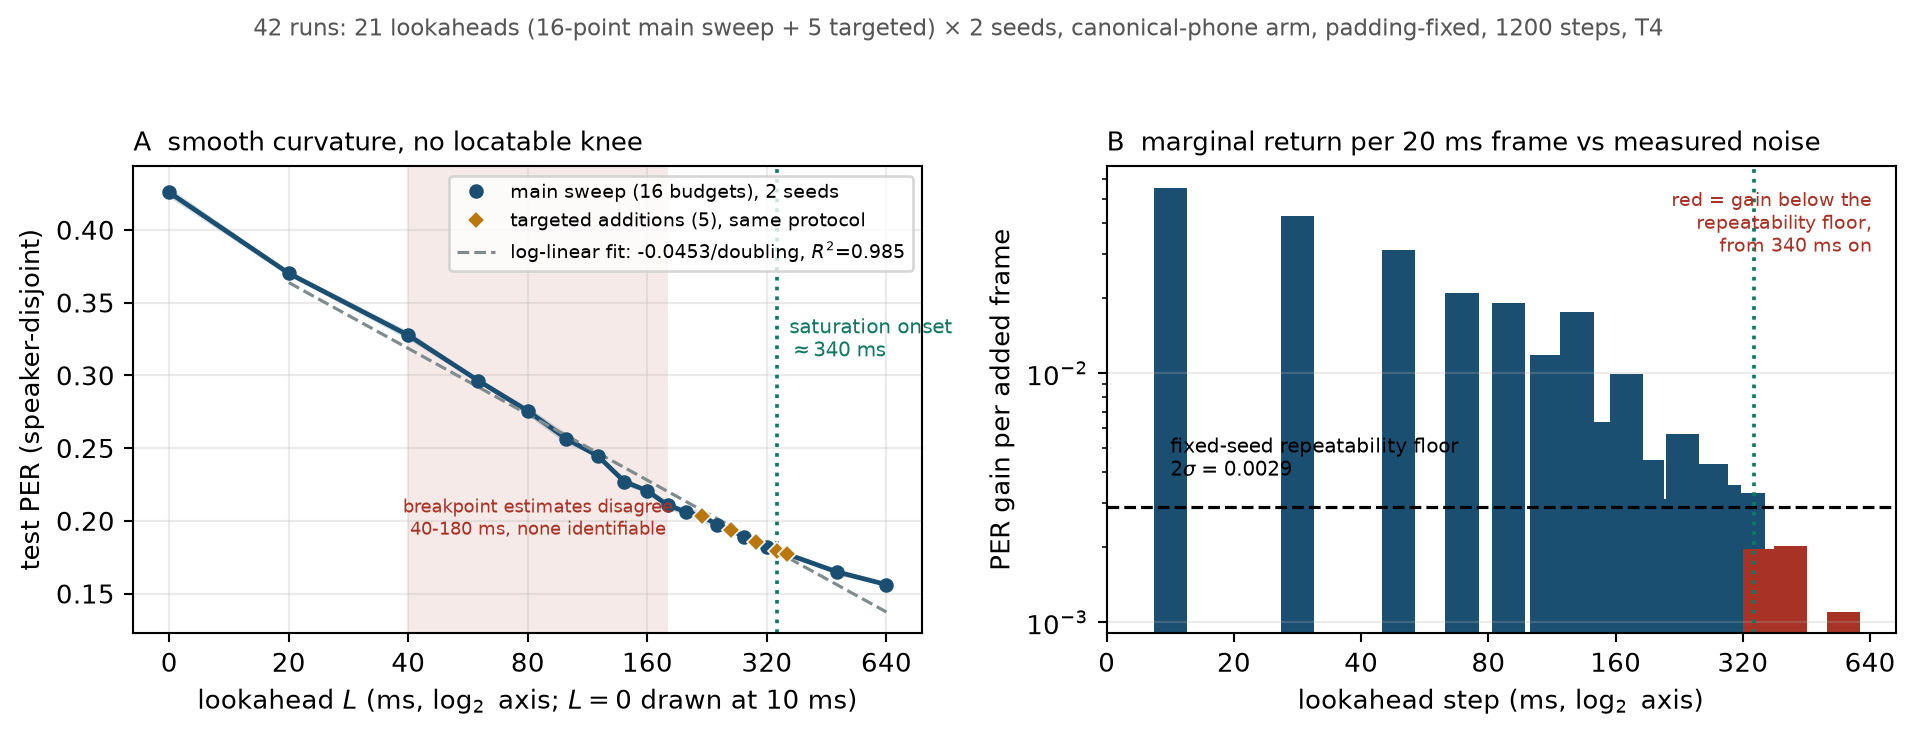
\includegraphics[width=\columnwidth]{fig_dense_no_knee.png}
\caption{Dense sweep, canonical-phone arm, 2 seeds: the 16-point main sweep
(circles) with the five targeted saturation-region additions (diamonds).
\textbf{Left:} smooth curvature; the shaded band spans the breakpoint estimates
produced by three defensible treatments of $L{=}0$, none identifiable.
\textbf{Right:} marginal return per added 20\,ms frame against the measured
$2\sigma$ floor; red bars are below it.}
\label{fig:dense}
\end{figure}

Canonical-phone-arm PER falls monotonically from $0.4256$ at $L{=}0$ to $0.1561$ at
$L{=}640$\,ms. Fitting $L\geq20$\,ms on $\log_2 L$ gives
\begin{equation}
\Delta\mathrm{PER} = -0.0452 \text{ per doubling},\quad R^2 = 0.983,
\label{eq:rate}
\end{equation}
over the 15 positive-lookahead points of the main sweep. The five budgets added
later to resolve the saturation region were sampled where the curve is
flattest, so we report the fit with and without them rather than silently
choosing one: including all 20 positive-lookahead conditions gives $-0.0453$
per doubling at $R^2=0.985$. Targeted sampling did not move the exchange
rate.

\textbf{There is curvature, and it is not localisable.} BIC prefers a
two-segment fit under all three axis treatments we tried
($\Delta\mathrm{BIC}=-31.0$, $-40.0$, $-46.5$ over all 21 budgets), which by
the usual thresholds~\cite{kassraftery1995} is strong evidence. But the
breakpoint lands at 40, 180 and 180\,ms respectively, and the bootstrap 90\%
intervals span 3.2, 2.6 and 3.2 octaves ($[40,360]$, $[60,360]$,
$[40,360]$\,ms). Twenty-one budgets do not yield an identifiable knee: the five budgets
added in the region where a knee would have to lie sharpened the evidence for
curvature without moving the breakpoint. The cause is structural: on a $\log_2(L{+}1)$ axis the $L{=}0
\rightarrow 20$\,ms gap is 4.39 units while every other gap is ${\approx}1.0$,
so a piecewise fit can be strongly biased toward placing a breakpoint just
past that gap even when the underlying curve has no localised knee.

\textbf{What we report instead} is the lookahead beyond which marginal return
falls below the measured floor. Because the original grid was 20\,ms-spaced
only to 200\,ms, we added the five budgets 220, 260, 300, 340 and 360\,ms
under identical settings, making the range 200--360\,ms fully 20\,ms-spaced.
The quantity below is therefore a per-\emph{observed}-step gain, not an average
over wider sampled intervals.

Gains run $+0.056$ (0$\rightarrow$20\,ms), $+0.021$ (60$\rightarrow$80) and
$+0.0045$ (180$\rightarrow$200). Against the measured floor of $0.0029$
(Eq.~\ref{eq:floor}), every observed 20\,ms step remains above it out to
340\,ms, at $1.1\times$ (200$\rightarrow$220), $2.0$, $1.3$, $1.5$, $1.2$,
$1.1$ and $1.1$. The observed $340\rightarrow360$\,ms increment is the first to
fall below it, at $0.7\times$, and the average per-20\,ms gain over the two
longer intervals that follow stays below it as well ($0.7$ over
$360\rightarrow480$ and $0.4$ over $480\rightarrow640$). We therefore place
\textbf{saturation onset at ${\approx}340$\,ms}. The wording is deliberate:
above 360\,ms the grid is not 20\,ms spaced, so a single sub-interval could in
principle exceed the floor without lifting its interval average, and what we
can state is the first sustained transition rather than a proven upper bound.

\textbf{This figure moves with the floor, and we report the sensitivity rather
than a single number.} Recomputing the onset at each end of the floor's
bootstrap interval moves it from 300\,ms (at $2\sigma=0.0034$) to 480\,ms (at
$0.0013$). This span is a sensitivity range induced by uncertainty in the
floor, not a confidence interval on a fitted saturation parameter. Under
the superseded $0.0044$ estimate it would have been 240\,ms, so the earlier
figure was an artefact of an over-conservative floor, not of the curve. The
gains between 200 and 340\,ms sit at only $1.1$--$2.0\times$ the floor, so this
is a region where returns become marginal rather than a sharp cutoff. Unlike a
knee, though, the quantity depends on the floor rather than on an axis
choice, and the floor is now measured with 12 degrees of freedom.

\begin{table}[t]
\centering\footnotesize
\setlength{\tabcolsep}{4pt}
\renewcommand{\arraystretch}{0.93}
\caption{Canonical-phone-arm PER against lookahead (mean of 2 seeds) and marginal
return per added 20\,ms frame, in units of the measured $2\sigma{=}0.0029$
floor (Eq.~\ref{eq:floor}). Below $1.0\times$, the gain from an additional
frame is smaller than the measured fixed-seed repeatability threshold. The grid is 20\,ms-spaced to 360\,ms; the final two rows
average over wider intervals.}
\label{tab:dense}
\begin{tabular}{rrrr}
\toprule
$L$ (ms) & PER & gain/frame & $\times$ floor \\
\midrule
0   & 0.4256 & --      & -- \\
20  & 0.3700 & 0.0556  & 19.2 \\
40  & 0.3275 & 0.0426  & 14.7 \\
60  & 0.2963 & 0.0312  & 10.8 \\
80  & 0.2754 & 0.0209  & 7.2 \\
100 & 0.2564 & 0.0190  & 6.6 \\
120 & 0.2446 & 0.0118  & 4.1 \\
140 & 0.2269 & 0.0176  & 6.1 \\
160 & 0.2206 & 0.0064  & 2.2 \\
180 & 0.2106 & 0.0099  & 3.4 \\
200 & 0.2062 & 0.0045  & 1.5 \\
220 & 0.2030 & 0.0031  & 1.1 \\
240 & 0.1973 & 0.0057  & 2.0 \\
260 & 0.1934 & 0.0039  & 1.3 \\
280 & 0.1891 & 0.0043  & 1.5 \\
300 & 0.1855 & 0.0036  & 1.2 \\
320 & 0.1823 & 0.0032  & 1.1 \\
340 & 0.1790 & 0.0033  & 1.1 \\
360 & 0.1770 & 0.0020  & \textbf{0.7} \\
480 & 0.1649 & 0.0020  & \textbf{0.7} \\
640 & 0.1561 & 0.0011  & \textbf{0.4} \\
\bottomrule
\end{tabular}
\end{table}

\textbf{Gain available beyond a small budget.} PER at $L{=}40$\,ms is
$0.3275$; at 340\,ms it is $0.1790$, a further relative reduction of 45.3\%,
and at 640\,ms the reduction is 52.3\%. In absolute terms, of the $0.2466$ PER
separating $L{=}0$ from $340$\,ms, the 40\,ms condition has captured $0.0981$,
or $39.8\%$. These budgets are per-layer values. By Table~\ref{tab:reach} the
40\,ms condition already draws on at least 220\,ms of future audio and the
340\,ms condition on at least 1.5\,s. The comparison therefore shows that, for
WavLM base+, the probe continues to benefit from future context well beyond
200\,ms. It does not measure what a system restricted to 40\,ms of end-to-end
lookahead forgoes, and no comparison with the budget of a published system is
implied. \S\ref{sec:encoder} further exhibits a backbone on which additional
context yields almost no improvement.

\subsection{The exchange rate does not transfer across encoders}
\label{sec:encoder}

Every number above is measured over one frozen backbone, which raises the question of whether the exchange rate is a property of the task or of the encoder. We
repeated the sweep on a second causalised encoder, wav2vec 2.0
base~\cite{wav2vec2}, holding the corpus, split, head, optimiser, step budget,
seed, chunk, lookback and matched lookahead grid fixed. The pretrained
backbone and the selected phonetic tap layer both differ, for reasons set out
below. The matched grid is $L\in\{0,20,40,80,160,320,640\}$\,ms, a subset of the main
sweep; fitted over this reduced grid the WavLM slope is $-0.0446$ rather than
the $-0.0452$ of Eq.~\ref{eq:rate}, which is why Table~\ref{tab:encoder}
differs slightly from \S\ref{sec:rq1}. Both encoders are causalised by the same
two patches and both pass the same truncation-based causality test.

\textbf{The layer must be matched by function, not by index.} Tapping
wav2vec 2.0 at layer 9, WavLM's phonetic layer, produces a degenerate
run: PER rises from $0.772$ at $L{=}0$ to $0.928$ and the training loss is
still falling steeply at step 1200. Probing the stack at $L{=}160$\,ms with
everything else fixed shows why (PER by layer: $0.402$ at 2, $0.411$ at 3,
$0.437$ at 4, $0.586$ at 6, $0.880$ at 8, $0.928$ at 9, $0.971$ at 10).
Decodability falls monotonically with depth: this encoder carries phones low
in the stack, and layer 9 is seven layers past its usable representation.
Matching two encoders by layer index is not matching them.

\textbf{How each layer was selected, and whether the choice drives the
result.} The two procedures are not symmetric and we state them plainly.
WavLM's layer 9 was fixed in advance from prior practice, before any lookahead
data existed, and was never re-selected. wav2vec 2.0's layer was chosen by the
probe above, which runs at $L{=}160$\,ms, inside the sweep it is later used
to interpret, so layer and lookahead sensitivity rest on partly overlapping
evidence. The concern this raises is that a layer picked mid-curve might
flatter or flatten the curve it is picked from. It does not here: re-selecting
on PER at $L{=}0$ alone, which is the endpoint the relative gain is measured
\emph{from} rather than a point on the response, returns the same layer
($0.4359$ at 2, $0.4590$ at 4, $0.5735$ at 6, $0.6940$ at 8). The comparison
below is therefore insensitive to which of the two criteria is used, though it
would be cleaner still to fix both layers by a pre-specified rule.

\begin{table}[t]
\centering\footnotesize
\setlength{\tabcolsep}{3.5pt}
\caption{Same sweep, second encoder, each tapped at its selected phonetic
layer, given in parentheses (\S\ref{sec:encoder}). Slope is PER per doubling
of lookahead, fitted over the matched grid. The two start with similar PER at
$L{=}0$ but exhibit markedly different lookahead responses.}
\label{tab:encoder}
\begin{tabular}{@{}lrrrr@{}}
\toprule
encoder & $L{=}0$ & $L{=}640$ & rel.\ gain & slope \\
\midrule
WavLM base+ (9)      & 0.4256 & 0.1561 & $+63.3\%$ & $-0.0446$ \\
wav2vec 2.0 base (2) & 0.4359 & 0.4189 & $+3.9\%$  & $-0.0015$ \\
\quad seed 7         & 0.4376 & 0.4265 & $+2.5\%$  & -- \\
\bottomrule
\end{tabular}
\end{table}

\textbf{Direction replicates; magnitude does not.} At the selected layer 2,
wav2vec 2.0 starts within $0.011$ PER of WavLM ($0.4359$ against $0.4256$) and
then barely moves: $3.9\%$ relative gain against $63.3\%$, and $-0.0015$ PER
per doubling against $-0.0446$. The log-linear fit that gives $R^2=0.989$ on
WavLM gives $R^2=0.099$ here, and the curve bottoms out at $L{=}160$\,ms
before rising again. The endpoint gain nonetheless exceeds the fixed-seed repeatability floor and
is reproduced at a second training seed.

\textbf{A second seed reproduces the weak, non-monotonic response.} The
comparison carries a headline claim, so we replicated it at a second training
seed on five budgets, including the 340\,ms onset that the first grid did not
sample. Seed 7 lands within $0.008$ PER of seed 1337 at every shared budget
($0.4376$/$0.4359$ at $L{=}0$, $0.4219$/$0.4169$ at 40, $0.4043$/$0.4004$ at
160, $0.4265$/$0.4189$ at 640; seed 7 gives $0.4155$ at 340, where seed 1337
sampled 320 and gave $0.4028$). Both curves reach their minimum at the same
$L{=}160$\,ms and both rise again by 640\,ms, so the non-monotonicity is a
reproducible feature of this encoder rather than one seed's noise. The endpoint
gain is $+2.5\%$ against $+3.9\%$: the effect is small in both seeds, with the
same non-monotonic pattern.

\textbf{Nor is it an artefact of the training budget.} A second seed cannot
rule out an optimisation effect the two seeds share: perhaps wav2vec 2.0's
lookahead conditions simply separate later. We therefore give this encoder the
same convergence check WavLM receives in \S\ref{sec:convergence}, at
$L\in\{0,160,640\}$\,ms to 6000 steps. Every condition improves ($0.4359
\rightarrow 0.3782$, $0.4004 \rightarrow 0.3361$, $0.4189 \rightarrow 0.3714$),
but they improve together, and the three-point ordering is unchanged: the
minimum remains at $L{=}160$\,ms and $L{=}640$ remains worse than it. Three
budgets test that ordering, not the full seven-point curve. The endpoint gain does not
grow with training; it \emph{shrinks}, from $+3.9\%$ to $+1.8\%$, while WavLM
at the same 6000 steps gains $+65.8\%$ on test PER
($0.4135\rightarrow0.1414$). Both encoder figures are test PER and so are
comparable to each other; Table~\ref{tab:conv} reports \emph{validation}
PER at checkpoints, on which the corresponding WavLM gain is $+63.8\%$. Five times the budget widens the gap
rather than closing it.

\textbf{This is not an artefact of tapping a shallow layer.} Layer 2 has had
substantially less contextual mixing than deeper layers, so the natural
objection is that there was less context to withhold and that sensitivity
would recover deeper in the stack. We do not observe that recovery. Relative gain from $L{=}0$ to $640$\,ms is $+3.9\%$ at layer 2,
$+5.4\%$ at 4, $+5.2\%$ at 6 and $-14.1\%$ at 8: flat across every layer
where the encoder can still decode phones, then negative. The expected trade-off is not observed.

\textbf{Tap depth and effective context.} Under the per-layer scheme the two
encoders do not receive the same future context at the same $L$: the WavLM
features pass through nine masked encoder layers and the wav2vec 2.0 features
through two, each followed by the four probe blocks. Part of the difference
between the two responses may therefore reflect effective context rather than
the encoder. The depth check above argues against this as the whole
explanation, since tapping wav2vec 2.0 at layers 4 and 6 increases the
effective context without restoring the sensitivity, but decodability also
falls with depth, so that check does not isolate the effect. The comparison
is between two configurations that differ in both encoder and effective
context.

Two encoders with similar zero-lookahead PER therefore differ by more than an
order of magnitude in endpoint relative gain, a statement that holds for
both wav2vec 2.0 seeds ($+2.5\%$ and $+3.9\%$ against $+63.3\%$). \textbf{The measured $-0.045$ PER per doubling is specific to the WavLM
base+ configuration tested here, and should be read as one encoder's operating
curve rather than as a fact about how much future context English phones
require.} The swap rules out treating the
measured WavLM exchange rate as a backbone-independent law, and it also shows that the detailed
shape need not carry over: WavLM's smooth diminishing-return curve has no
counterpart in wav2vec 2.0's weak, non-monotonic one. We do not run the
breakpoint and axis-perturbation analysis of \S\ref{sec:rq1} on a curve that
is not monotone, so we make no knee claim about it either way. Every positive
quantity here, the exchange rate, the saturation onset and the gain available beyond a small budget, should therefore be re-measured on whatever backbone a
system actually deploys. Whether the gap traces to pretraining scale (960\,h against
94\,k\,h), to WavLM's denoising and speaker-conditioned objectives, or to
something else is not something a two-encoder comparison can decide.

\subsection{RQ2: the pre-specified manner grouping does not predict lookahead benefit}
\label{sec:rq2}

We fixed this prediction in code before the hypothesis outputs it is tested on
were generated. The grouping, and the rationale for it, sit in
\texttt{eval/phoneme\_analysis.py} at commit \texttt{c5066dc} of the public
repository (2 Aug 2026),\footnote{\url{https://github.com/Dipeshtripathi13/streaming-fac-lookahead/commit/c5066dc}}
seven days before the hypothesis dumps were committed (\texttt{b66d0a5}, 9 Aug
2026). We are precise about what this does and does not establish. It is not a
registered pre-registration, and we do not call it one: git author and
committer dates are set by the
committing machine and history can be rewritten, so the chronology is a claim
about our repository rather than third-party attestation. What it does give a
reader is the \emph{content} of the prediction, verbatim and inspectable,
including the class assignment and the reasoning we offered for it at the
time. The current public history is consistent with the prediction preceding
the outputs it is tested on, but consistency is the most that can be claimed:
this is not immutable third-party timestamping. The prediction was
that vowels and approximants break first while stops, fricatives, affricates
and nasals would survive short lookahead. The reasoning was that vocalic
identity is carried by formant movement across a syllable nucleus that is tens
to hundreds of milliseconds long. Peterson and Lehiste measured English
syllable nuclei at roughly $80$--$250$\,ms \cite{petersonlehiste1960}, a range
consistent with the vowel durations later reported over 139
talkers \cite{hillenbrand1995}. The second half of the reasoning was that this
movement is criterial rather
than incidental, since even nominal monophthongs are identified better from a
trajectory than from a steady-state slice \cite{nearey1986}, with glides and
diphthongs differing from vowels in rate of formant change rather than in
kind \cite{lehistepeterson1961}. Stops, fricatives and affricates were placed
in the comparison group because their defining cues are comparatively
localised: stop place is signalled by brief formant transitions to a
locus \cite{delattre1955} and is recoverable from a short-time spectrum at the
release \cite{stevensblumstein1978}, so a narrow window should suffice. Nasals
were assigned to the same group under the same short-context prediction, but
the acoustic argument above is strongest for the obstruent classes and we do
not claim it extends cleanly to nasals. We record this asymmetry as it stood
when it was specified rather than reconstructing a stronger rationale after the
grouping failed. Nasals in fact gain the most of any class
(Table~\ref{tab:h2}). Testing this on 42{,}255 unique reference-phone tokens evaluated across seven
lookahead conditions (295{,}785 phone--condition observations), with each
substitution or deletion charged to the class of the \emph{reference} phone:

\begin{table}[t]
\centering\footnotesize
\setlength{\tabcolsep}{4pt}
\renewcommand{\arraystretch}{0.93}
\caption{Relative error-rate reduction, $L{=}0\rightarrow640$\,ms. B =
pre-specified as breaking first, S = as surviving. Intervals are
percentile bootstrap over the six test speakers, not over phone
tokens. The predicted grouping does not order the data.}
\label{tab:h2}
\begin{tabular}{llrcr}
\toprule
& class & rel.\ gain & 95\% CI & ref.\ phones \\
\midrule
S & nasal        & 0.716 & [0.668, 0.779] & 4\,020 \\
B & approximant  & 0.700 & [0.628, 0.774] & 4\,575 \\
S & fricative    & 0.687 & [0.608, 0.774] & 7\,659 \\
B & vowel (mono) & 0.673 & [0.595, 0.767] & 13\,008 \\
B & vowel (diph) & 0.654 & [0.577, 0.758] & 4\,824 \\
S & stop         & 0.615 & [0.550, 0.689] & 7\,071 \\
S & affricate    & 0.525 & [0.397, 0.633] & 1\,098 \\
\bottomrule
\end{tabular}
\end{table}

Group means differ in the predicted direction ($0.676$ vs $0.636$), but that is
the weakest available reading and four stronger checks fail. The effect size
is $0.66$: the between-group difference ($0.040$) is smaller than the pooled SD
across classes ($0.060$). The surviving group's \emph{internal} spread is
$0.190$, which is $4.7\times$ the between-group difference. And 5 of 12 pairwise
orderings are violated, with nasals out-gaining all three breaks-first classes.

\textbf{Under speaker-level resampling the difference is not distinguishable
from zero.} The 42{,}255 tokens per condition are not independent: they are
nested in six speakers, and the claim at issue is about accented speech, for
which the independent replicate is a talker rather than a phone. Resampling
speakers rather than tokens (2000 draws, Table~\ref{tab:h2}) puts the
between-group difference at $+0.040$ with a 95\% interval of
$[-0.010, +0.101]$, which \textbf{includes zero}. Every individual class gain
stays substantial, with the intervals in Table~\ref{tab:h2} between $0.40$ and
$0.78$; what fails to separate from zero is the \emph{grouping}. Token-level intervals
would have been roughly an order of magnitude narrower and would have declared
this difference significant, which is the error the clustering avoids. The same
procedure applied to RQ3 (Sec.~\ref{sec:rq3}) resolves the larger interaction
there, so the estimator is not uniformly uninformative at six speakers, though
that alone does not establish power for an effect this small.
A cluster bootstrap over six clusters leans on asymptotics that six clusters do
not supply, so we add the non-asymptotic companion: recomputing the difference
with each speaker removed in turn gives $+0.0217$ to $+0.0592$ (pooled
$+0.0401$). No single talker drives the estimate, since the sign is stable
across all six drops, but the entire leave-one-out range also sits inside an
interval that contains zero, so the verdict does not change.

\textbf{The pattern does not hold within L1 either, but that split cannot carry
weight.} Splitting by native language, the ratio of group gains straddles
unity: Vietnamese $1.23$, Korean $1.19$, Arabic $1.08$, Spanish $1.02$,
Hindi $0.99$, Chinese $0.92$; requiring both the gain ratio and the mean slope
to move in the predicted direction, only 3 of 6 qualify (Spanish clears the
gain criterion but not the slope one). The reversals show that the pooled
ordering is not consistent across the six held-out speakers, each of whom
carries a distinct L1 label.
The deeper limitation is that in the speaker-disjoint test split \emph{each L1
is represented by exactly one speaker} (ABA, LXC, SVBI, HJK, EBVS, PNV), so L1
and talker are perfectly confounded: this table cannot separate a language
effect from an individual one, and every ``by-L1'' row is equally readable as one
speaker's idiosyncrasy. We report it as a consistency check, not as evidence
about native language.

\textbf{H2 is not supported.} Not because lookahead fails to help vowels, since
every class improves 52--72\% relative, but because the pre-specified manner
grouping does not reliably order lookahead benefit.

\textbf{Reweighting each error by a proxy for its acoustic cost does not rescue
it.} PER charges every error exactly $1.0$, so the natural objection is that
the grouping is sound and PER simply mis-weights it: a substituted vowel and a
substituted stop cannot sound equally wrong. We test that directly.

Each utterance's canonical phone string is synthesised with a single fixed
voice and force-aligned to its own synthesis using an espeak-IPA CTC model,
giving a time span per reference phone. The hypothesis string is synthesised
with the same voice and DTW-aligned to the reference, and the spectral
distortion inside each reference phone's own span is charged to that phone's
class. Localisation matters here: a VITS-class synthesiser is globally coupled,
so changing one phone perturbs the whole utterance and a whole-utterance
distortion cannot be attributed to a single phone. The per-phone span from
forced alignment is what makes the measurement local at all.

Synthesis must also be deterministic. Piper defaults to
$\mathrm{noise\_scale}=0.667$ and $\mathrm{noise\_w}=0.8$, under which the same
phone string renders differently on each call: self-distortion is $244.8$
against $277.6$ for a genuine one-phone change, so roughly 88\% of an apparent
``cost of an error'' would be synthesis noise. Both terms are zeroed, giving
bitwise-identical renderings, and the analysis refuses to run otherwise.

Two sanity checks support the measure before it is used, and the verdict is suppressed if
validation fails: phones the sequence metric scores as incorrect carry
$1.72\times$ the distortion of correct ones ($86.8$ versus $50.5$), and mean
distortion falls monotonically with lookahead ($71.4$ to $46.9$, $-34\%$).

The verdict is unchanged. Acoustic weighting does move
in H2's favour, with effect size $0.607 \rightarrow 0.756$ and ordering
violations $4/12 \rightarrow 2/12$ against the sequence metric on the same
utterances, but not far enough to clear the pre-specified threshold of $1.0$, and the
failure has the same shape as before: the ``survives'' group's internal spread
($0.120$) is $3.5\times$ the difference between the groups ($0.034$), and a
nasal again out-gains a diphthong; the per-class figures are in the
repository. So this particular equal-cost objection is not supported by the synthesised
distortion analysis; it does not exclude weightings this proxy cannot see,
notably trajectory errors at correctly identified phones.



One explanation does remain open, and it is not the one this test closes. Both
signals here are TTS renderings of phone strings, so the synthesiser produces
canonical formant trajectories for whatever string it is given. This measures
the cost of getting a phone's \emph{identity} wrong; it says nothing about a
wrong trajectory for a phone whose identity is right. That still needs real
converted audio against a native rendition (\S\ref{sec:remaining}). The sample
is also far smaller than the sequence-level test, at 1451 unique reference
phones per acoustic condition against 42{,}255 per sequence condition, and
is weighted accordingly.

\subsection{RQ3: canonical-phone prediction benefits more from lookahead than realized-phone transcription}
\label{sec:rq3}

Identical architecture, capacity, data order, seed and step count; the two arms
differ only in the target tensor. Endpoint gain $L{=}0\rightarrow640$\,ms is
$-0.2695$ (63.2\% relative) for canonical-phone prediction against $-0.1893$
(42.8\%) for realized-phone transcription, a paired difference of $+0.0802$
across the three seeds ($\mathrm{sd}=0.0035$, $t(2)=39.7$, $p=6.3\times
10^{-4}$, 95\% CI $[+0.0715, +0.0889]$). With three seeds the interval is wide
in principle and narrow here only because the seed-to-seed spread is small
relative to the effect.

\textbf{The dense grid replicates this, and sharpens it.} Running the full
16-lookahead $\times$ 2-seed sweep on the transcription arm as well puts both
arms on the same dense grid. The endpoint gains
reproduce the 7-point result almost exactly, at 63.3\% for canonical-phone
prediction against
43.5\% for transcription, against 63.2\% and 42.8\% before, in an
independent set of training runs on a denser grid, though on the same corpus
and test split; per-condition values for both arms are in the repository.
The exchange rates separate cleanly:
\begin{center}
canonical-phone $-0.0452$ vs transcription $-0.0292$ PER per doubling,
\end{center}
$R^2 = 0.983$ and $0.984$ respectively, so \textbf{canonical-phone prediction
buys $\mathbf{1.55\times}$ as much per doubling of lookahead}.

The effect is clearer in the between-arm gap than in the absolute levels. At
$L{=}0$ the two arms have similar PER ($0.4256$ vs $0.4427$, a gap of
$0.0171$); by
$L{=}640$\,ms the gap is $0.0939$, \textbf{5.5$\times$ wider}. It widens in
13 of 15 adjacent steps, and the transcription arm is worse at 16 of 16
lookaheads, every one by more than the $0.0029$ floor.

The arms differ in their target tensor, which carries more than the task: label
entropy, sequence length and annotation noise move with it. We therefore repeat
the test within a single canonical-phone model, holding the target
representation and the model fixed; the two position subsets can of course
still differ in composition and baseline difficulty, which is what the controls
below address.

\textbf{Defining a canonical-deviation position.} The \texttt{g2p} and
\texttt{ipa} strings are not positionally aligned and differ by substitutions,
deletions and insertions, so a position-$i$ comparison is not available. We
align them with Levenshtein backtrace under unit substitution, insertion and
deletion costs, and index every quantity by the \emph{canonical}
(\texttt{g2p}) sequence. A position is a canonical-deviation position when its
aligned operation is a substitution or a deletion; an insertion in the
\texttt{ipa} stream consumes no canonical position and is skipped. Model errors
are charged to canonical positions by the same rule, aligning \texttt{g2p}
against the CTC hypothesis, so that deviation status and error status index the
same sequence. Where ties occur the backtrace prefers substitution over
deletion over insertion, making the mapping deterministic. One consequence
belongs with the result: because everything is indexed to canonical positions,
realized-phone insertions are excluded from this analysis, so it covers the
substitution and deletion deviations rather than every way the two strings can
differ. This is the
convention used throughout the paper, including the manner-class analysis of
\S\ref{sec:rq2}.

Splitting canonical positions this way, the exchange rate is $-0.0520$ PER
per doubling at canonical-deviation positions against $-0.0394$ at matching ones,
a factor of $\mathbf{1.32}$ from the same model on the same utterances. That
converges with the $1.55\times$ between arms. One caveat belongs with it: in
\emph{relative} terms the ordering reverses ($51\%$ against $71\%$), because
canonical-deviation positions start far harder ($0.590$ against $0.354$) and the
gap between the two widens with lookahead. Absolute PER decreases faster at canonical-deviation positions, although these
positions begin substantially harder and show a smaller relative reduction.

\textbf{The interaction survives two controls.} Those positions are not a
random subset: they differ in baseline difficulty, phone composition and
distribution over speakers. Treating 42{,}255 phone tokens nested in six
speakers as independent would substantially overstate precision by ignoring
within-speaker dependence, so we bootstrap over
\emph{speakers}: the slope difference is $-0.0127$ with a 95\% CI of
$[-0.0211, -0.0069]$, excluding zero, and deviation positions are steeper in
2000 of 2000 resamples. Leave-one-speaker-out agrees and is not asymptotic:
dropping each talker in turn gives $-0.0152$ to $-0.0095$, negative in all six
cases and never approaching zero. The result is also insensitive to how
ambiguous alignments are resolved: re-running with the backtrace preferring
deletion over substitution moves the slope difference from $-0.0127$ to
$-0.0131$ (ratio $1.32$ to $1.33$, CI $[-0.0218, -0.0071]$, still 26 of 35
phones in the same direction), so the result does not depend on the tie-breaking rule. Recomputing the difference \emph{within each reference
phone} and pooling gives $-0.0098$, steeper in 26 of 35 phones, so phone
composition accounts for roughly a quarter of the raw gap but not the effect.
We report this as an association under matched conditions, not as evidence
that \texttt{g2p}$\neq$\texttt{ipa} positions are exclusively where accent
resides: such positions also include pronunciation variants, reductions and
annotation error.

One secondary observation follows: neither arm yields a locatable knee
(breakpoints move to $[40, 240, 160]$\,ms across axis treatments for
transcription, against $[40, 180, 180]$ for canonical-phone prediction), so
\S\ref{sec:rq1}'s structural conclusion is not an artefact of the
canonical-phone arm. We do not compare saturation onsets between the arms: the five budgets
added over 200--360\,ms to locate it were run on the canonical-phone arm only, so
the transcription arm lacks the resolution the comparison would need. The
transcription arm's own curve is just as log-linear, with a shallower slope.

A complementary within-run measure is the \emph{preference margin}, PER
against the other arm's labels minus PER against its own. It grows
monotonically in 3/3 seeds for the canonical-phone arm ($+0.032$ at $L{=}0$ to $+0.099$ at 640\,ms; 18/18
adjacent step $\times$ seed comparisons positive) while the transcription
control is 0/3 monotone and drifts \emph{down} ($-0.0103$). The margin is a difference rather than a level, which makes it robust to the offset discussed in \S\ref{sec:lessons}.

\subsection{\texorpdfstring{\tbuf{}}{t\_buf}: jitter measured, I/O not}

\tbuf{} splits into a jitter term and an I/O term. The first is measured; the
second resisted three separate attempts, and we report that rather than
substitute a number.

\textbf{On the M4 test platform, measured jitter is negligible relative to the
other latency terms.} Two independent 30\,s duplex runs on the M4 at
40\,ms blocks give required jitter buffers of $0.14$ and $0.08$\,ms, p99
callback lateness ${\approx}0.06$\,ms, zero over- or underruns, and clock drift
below $1.3\times10^{-4}$\%. On this platform the jitter safety margin
contributes nothing meaningful to the budget.

\textbf{The I/O term is unmeasured, and the reason is instructive.} Three
attempts failed, each for a different reason, and we report that rather than
substitute a number. An acoustic loopback was defeated by platform echo
cancellation: all 20 repetitions fell below the correlation threshold, and
captured level was \emph{invariant} to output amplitude, so a louder probe
could not help. The driver-reported figure is not a substitute, being
identically $201.69$\,ms in excess of the requested block at both 10 and
20\,ms; a quantity invariant to a doubling of the block size is not measuring
the block. A digital loopback through a virtual audio device returns a signal
so weak that the detection threshold has to be lowered until repetitions pass,
which yields p50 $206$\,ms against p90 $491$\,ms. We reject that as
threshold-dependent rather than representative, and such a device would in any
case measure its own buffering. Closing this term needs a wired loopback
through real converters, or a platform without echo cancellation in the path;
the full traces are in the repository.

\section{Measurement audits and failure modes}
\label{sec:lessons}

\textbf{A padding error changed the shape of the curve.} A masked block handed a
zero-padded hidden-state tensor to a depthwise convolution and feed-forward
that do not respect the key-padding mask. The correction was not a constant
offset: it grows with lookahead, from $-0.014$\,PER at $L{=}0$ to $-0.086$
at 320\,ms, $16.4\times$ the noise floor. The buggy curve therefore
\emph{understated} the benefit of lookahead, biasing the central quantity of
RQ1. A constant offset would have cancelled in every within-run comparison;
this did not. Every number reported in this paper was regenerated after the
fix.

\textbf{A forced one-breakpoint estimator returns a breakpoint even when no localised knee
exists.} $\Delta$BIC cannot distinguish ``there is a knee'' from ``piecewise
fits a curve better than a line''. Identifiability has to be tested by
perturbing the axis and bootstrapping the location, not inferred from
$\Delta$BIC alone. Our synthetic check reproduces the artefact exactly: on a
curve that is log-linear for $L\geq20$ with $L{=}0$ off the extrapolation,
including $L{=}0$ yields $\Delta\mathrm{BIC}=-39$ and a confident ``knee at
40\,ms'', while dropping it yields $+5$ and no knee at all. An earlier
maximum-distance-to-chord estimator reported ``knee at 160\,ms, bootstrap 95\%
CI $[160,160]$'' on this data, a tight interval around a plausible value,
tight precisely \emph{because} the curve is smooth and every resample of a
log-linear curve is also log-linear.

\textbf{An analysis that buckets unmatched symbols into ``other'' will produce
confident output on the wrong alphabet.} Our phoneme-class map was keyed on
ARPAbet; the sweep emits IPA. Applying one to the other sent 57\% of reference
tokens, including \emph{every} vowel and \textipa{/\*r/}, to ``other'',
and still printed per-class slopes, an H2 verdict and a by-L1 table. No error was raised. The guard is to assert coverage rather than infer it from the absence
of an exception, which the analysis now does.

A fourth attempt, a TTS-counterfactual substitute for forced alignment, was
built and rejected before producing any reported number; it is documented in
the repository.

\section{Limitations}
\label{sec:remaining}

\textbf{The lookahead axis of the reported sweeps is nominal.} The sweeps
used a per-layer mask, under which the effective future context exceeds $L$
by the amounts in Table~\ref{tab:reach}. The measured error rates, and the
comparisons between arms at equal $L$, remain valid as functions of the
nominal value, but no budget
reported here should be read as an end-to-end algorithmic delay, and the
cross-encoder comparison is confounded with tap depth.

\textbf{Every quality result here is phone-level, not perceptual}, and this is
a phone-translation probe rather than an end-to-end FAC system: the
latency--accuracy relation reported here need not transfer to synthesis,
prosody, speaker similarity or perceived accentedness. We do not conduct a perceptual
study because the phone-sequence outputs are not valid FAC stimuli: synthesised
from bare phone strings, they lack the lexical, prosodic and acoustic structure
required to judge naturalness or accentedness. This is a property of the
stimuli rather than of the budget. Training is 1200 steps at fixed budget
over a frozen encoder, a comparison at matched budget rather than at
convergence, though \S\ref{sec:convergence} shows the ranking and exchange
rate hold to $5\times$ that budget; the dense sweep has two
seeds per arm. Its repeatability threshold now comes from a deliberate
four-condition $\times$ four-repeat experiment with a bootstrap interval, but
that threshold is global while the per-condition $\sigma$ it pools varies by a
factor of $3.5$, so marginal decisions near the threshold should be treated as
approximate. \tbuf{}'s I/O term is unmeasured, and compute is characterised on Apple
Silicon and ARM64 Linux only. The encoder comparison in
\S\ref{sec:encoder} compares two pretrained encoder checkpoints. The wav2vec
2.0 result is replicated at a second training seed and re-checked at 6000
steps, while the WavLM curve rests on the seeds of the main sweep; that is
enough to show the exchange rate does not transfer, but not to attribute the
gap to pretraining scale, objective or architecture; and the layer-selection protocols are not
fully symmetric: WavLM's layer 9 was fixed a priori from prior practice,
whereas wav2vec 2.0's was selected by a phonetic probe at one lookahead, though
re-selection at $L{=}0$ returns the same layer.

\section{Conclusion}

A lookahead budget describes a streaming model only if the output of the
complete model depends on no more future input than the budget states. Two
conditions for this were found not to hold by default: masking self-attention
leaves a pretrained encoder non-causal, and a lookahead mask applied in every
layer compounds, so that a nominal 40\,ms corresponded here to at least
220\,ms. Both are detected by simple input-perturbation tests, and both have
direct remedies. For the causal WavLM phone-translation probe under per-layer
lookahead, future context reduces PER at an approximately log-linear average
rate of ${\approx}0.045$ per doubling, with no identifiable knee and
measurable returns out to a nominal $340$\,ms, at least 1.5\,s of effective
context. That rate, however, is measured
over one backbone: a second causalised encoder with similar zero-lookahead PER
shows only a $3.9\%$ relative endpoint PER reduction from $0$ to $640$\,ms
against $63.3\%$ for WavLM, and $1.8\%$ when both are trained to 6000 steps
(\S\ref{sec:encoder}). Neither the magnitude nor the detailed shape of the
response transfers across the two encoders tested, so future-context budgets
should be characterised for the deployed representation rather than inherited
from another backbone. Increasing lookahead changes algorithmic latency substantially while only weakly affecting measured per-chunk compute over the tested range,
though throughput must still satisfy $\tcmp<c$
(Eq.~\ref{eq:rtf}) to run at all.

\section{Acknowledgements}

This work received no external funding and used no institutional compute: GPU
results are from free-tier Google Colab (Tesla T4), CPU results from consumer
hardware. Thanks to the maintainers of L2-ARCTIC, WavLM, sherpa-onnx and
Piper, whose public releases made a study of this scope possible.

\section{Compliance with ethical standards}

This work used only the publicly released L2-ARCTIC corpus and involved no new
participant recruitment, interaction or data collection. No listening study was
run and no claim about perceived accentedness is made. The author declares no
competing interests.

\bibliographystyle{IEEEtran}
\bibliography{refs}

\end{document}
